\begin{center}
  \section{\capitalisewords{Neuromorphic Computing Chips Inspired by the Human Brain}}
  Soumyadeep Sengupta, 1$^{st}$ Year, ECE
\end{center}
\vspace{-0.18em}

\setcounter{figure}{0}
\setcounter{table}{0}

\begin{multicols}{2}
  \begin{abstract}
    \bfseries
    Artificial Intelligence revolution is built on an unstated inefficiency, while the human brain performs complex discernment on approximately 20 watts, a state-of-the-art GPU draws up to 700 watts for similar workloads. Neuromorphic computing addresses this basic inconsistency by replicating the framework of biological neural networks directly in hardware by integrating memory and computation. Running only on incoming spike events, and learning through local synaptic rules rather than global backward propagation of errors. This report goes over the entire neuromorphic pipeline, from the biological neuron's threshold-firing mechanism to Spiking Neural Networks (SNNs) trained using surrogate gradient methods and Model Fusion Technology (MFT), continuing into silicon implementation on Intel's Loihi 2 and the billion-neuron Hala Point
    system. We go over the 2024--2025 state-of-the-art benchmarks, including SpikeYOLO achieving 66.2\%
    mAP@50 on COCO with \(5.7\times\) energy efficiency over equivalent ANNs, and Advanced SpikingYOLOX
    leveraging 2D-Spiking Transformers for object detection at ACM MM 2025 that confirm SNNs have crossed
    from research interests to competitive engineering. The 2026 University of Cambridge hafnium oxide
    memristive synapse breakthrough, providing a 70\% energy reduction using standard CMOS-compatible
    materials, is analysed alongside the critical integration challenge of linking spike-domain hardware with real-
    valued deep learning pipelines. With the neuromorphic market projected to reach \$61.48 billion by 2035 at a
    33.32\% CAGR, and neuromorphic chip patents rising 401\% in 2025 alone, this report demonstrates that computing modelled by the human brain is not a future possibility, it is an engineering reality.

    \vspace{1em}
    {\justifying\noindent\textbf{Keywords:} Neuromorphic Computing, Spiking Neural Networks, Surrogate Gradient, MFT Training, SpikeYOLO, SpikingYOLOX, Memristor, ANN-to-SNN Conversion, Loihi 2, Hala Point, Event-Driven AI.\par}
  \end{abstract}

  \subsection*{\centering\uppercase{INTRODUCTION}}
  There is a strange contradiction at the base of modern AI. The field's greatest ambition to replicate human intelligence is pursued using hardware fundamentally opposite to the organ it seeks to replicate. The human brain processes information across 86 billion neurons connected by 100 trillion synapses, running on roughly 20 watts of cellular power. The NVIDIA H100 GPU, today's AI workhorse, draws up to 700 watts under full load. At data-centre scale, this gap becomes critical. Global AI infrastructure is projected to consume 1,000 TWh of electricity yearly by 2026 comparable to Japan's total national energy consumption.

  \noindent
  This is not merely an environmental concern, it is an engineering ceiling. As AI models scale toward hundreds of trillions of new limits, power consumption threatens to become the front running issue on further capability growth. The solution, many researchers argue, has been operating inside human skulls for millions of years.

  \noindent
  Neuromorphic computing, first theorized by Carver Mead at Caltech in the 1980s proposes the idea of building chips that mirror biological neural networks structurally and programmatically. Unlike conventional von Neumann architectures, which continuously shift data between separate memory and processing units, neuromorphic systems co-locate computation and storage. These activate only on spike events, and learn
  through local synaptic adaptation. Between 2024 and 2026, the initial model crossed a decisive onset from laboratory demonstration to competitive benchmarks, from exotic materials to CMOS-compatible fabrication, and from academic precursor to the world's largest deployed AI system by neuron count.

  \subsection*{\centering\uppercase{Biological Foundations: From Neuron to Circuit}}
  \subsubsection*{Threshold-Fired Spike Coding}
  A biological neuron brings together electrochemical inputs across its dendritic membrane. Only when
  accumulated charge crosses a critical upper limit, does it emit a different action potential. It sends a
  spike down its axon to connected neurons. This \textbf{all-or-nothing}, action-driven mechanism encrypts
  information in spike timing and rate, not continuous amplitude. The result stands out as zero
  computation during silence, and information processing only when something in the environment
  actually changes.

  \noindent
  Neuromorphic chips replicate this using \textbf{Leaky Integrate-and-Fire (LIF)} neurons. The most widely
  implemented spiking neuron model. Each LIF unit accumulates input charge as membrane
  potential \(V_m\), decays it with a leak term \(\tau\), and emits a spike when \(V_m\) exceeds threshold \(V_{\mathrm{th}}\). It
  immediately resets afterwards.

  \noindent
  The \textbf{Dynamic Threshold LIF (DT-LIF)} variant, suggested in 2025, dynamically adjusts \(V_{\mathrm{th}}\) based on
  incremental membrane potential, improving inference speed and increasing object detection accuracy
  on the \textbf{Prophesee Gen1} dataset by \textbf{25.2\%} over standard LIF implementations.

  \subsubsection*{Synaptic Plasticity: The Learning Synapse}
  Biological synapses strengthen or weaken through \textbf{Spike-Timing-Dependent Plasticity (STDP)}: if a
  presynaptic neuron fires just before a postsynaptic one, the synapse strengthens after, it weakens. This
  local, unsupervised rule requires no global loss function and no backpropagation signal. Hence, the
  synapse is the learning unit. Memristive (devices or materials that exhibit ``memristance'') device are
  two-terminal elements whose resistance history mirrors synaptic weight history are the hardware
  implementation of this principle.

  \subsection*{\uppercase{Training SNNs: The Surrogate Gradient Revolution}}
  \subsubsection*{The Non-Differentiability Problem}
  For a long period of time, SNNs could not be trained with standard backpropagation. This issue occurred
  because the spike function, a binary step has zero gradient almost everywhere. Hence, making gradient-based
  weight updates that were mathematically undefined. This "dead gradient" problem restricted SNNs to basic
  architectures trained by biologically-motivated but limited local rules like STDP.

  \noindent
  The field's breakthrough came through \textbf{surrogate gradient methods}, replacing the non-differentiable spike
  function with a smooth, differentiable approximation during the backward pass only, while preserving true
  binary spikes during forward computation. This allows deep SNNs to be trained end-to-end with
  backpropagation-through-time (BPTT), unlocking architectures as deep as ResNet-34 on large-scale datasets.

  \subsubsection*{Model Fusion Technology (MFT): Best of Both Worlds}
  The 2024--2025 state-of-the-art training framework is \textbf{Model Fusion Technology (MFT)}, which hybridizes two previously competing approaches:
  \begin{itemize}
    \item \textbf{Direct Training (STBP):} Trains SNNs from scratch using surrogate gradients high accuracy but slow convergence and high time-step requirements.
    \item \textbf{ANN-to-SNN Conversion:} Pre-trains an ANN, then converts activations to spike rates fast but incurs large time-step overhead (100--1000+ steps) for accurate conversion.
  \end{itemize}
  MFT fuses both an ANN backbone is pre-trained conventionally, a \textbf{Batch-Matched Integrate-and-Fire (BM-
  IF) neuron} simplifies the conversion stage and reduces conversion error, and surrogate-gradient fine-tuning
  then refines the hybrid network. Results on this approach are striking:

  Table~1 compares MFT-based SNN and ANN-to-SNN conversion on key benchmarks.

\begin{center}
\vspace{-0.5em}
\begin{minipage}{0.98\columnwidth}
\centering
    \captionof{table}{MFT-based SNN vs. ANN-to-SNN conversion on key benchmarks}
    \scriptsize
    \setlength{\tabcolsep}{3pt}
    \renewcommand{\arraystretch}{1.25}
    \begin{tabular}{@{}>{\RaggedRight\arraybackslash}p{0.28\columnwidth}>{\RaggedRight\arraybackslash}p{0.31\columnwidth}>{\RaggedRight\arraybackslash}p{0.31\columnwidth}@{}}
      \toprule
      \textbf{Metric} & \textbf{ANN-to-SNN Conversion} & \textbf{MFT-based SNN} \\
      \midrule
      Inference time steps & \(512\text{--}1250\times\) baseline & \(1\times\) (\(512\text{--}1250\times\) reduction) \\
      ImageNet-1K Accuracy & \(\sim 65\%\) (SOTA) & 67.38\% (new SOTA) \\
      Remote sensing (UCM) & \(\sim 97\%\) & 99.62\% \\
      Remote sensing (AID) & \(\sim 96\%\) & 98.81\% \\
      Convergence speed & Slow (STBP) & Significantly faster \\
      \bottomrule
    \end{tabular}
\end{minipage}
  \end{center}

  Additionally, \textbf{Differential Coding} (ICML 2025) advances ANN-to-SNN conversion further by
  transmitting changes in spike rate information rather than absolute rates---reducing total spike count and
  energy while achieving state-of-the-art accuracy, including \textbf{75.12\% on ImageNet with only 4-time steps}.

  \subsection*{\uppercase{Object Detection: SNNs Enter the Real World}}
  \subsubsection*{SpikeYOLO (ECCV 2024)}
  SpikeYOLO, presented at ECCV 2024, demonstrated that naive conversion of YOLO-series architectures to
  spiking equivalents causes spike degradation---complex module designs suppress spike propagation through
  deep layers. SpikeYOLO resolved this by simplifying the backbone with meta SNN blocks optimized for sparse
  spike flow and designing a new neuron activating integer values during training while extending virtual
  timesteps during inference. On the COCO dataset, it achieved 66.2\% mAP@50, which is 15.0 percentage points above the prior SNN
  state of the art; on the Gen1 neuromorphic dataset, it achieved \(5.7\times\) greater energy efficiency than an equivalent ANN.

  \subsubsection*{Advanced SpikingYOLOX (ACM MM 2025)}
  Advanced SpikingYOLOX extended SNN-based detection further using two architectural innovations: Spike-based Partial Self-Attention (SPSA), which selectively applies attention to high-information spike channels
  reducing computational overhead, and a 2D-Spiking Transformer that processes spatial and temporal spike
  dimensions jointly. Together, these bring transformer-class feature extraction into the spike domain---
  delivering ANN-competitive accuracy while retaining neuromorphic energy efficiency. This paper effectively
  closes the argument: on event-driven, temporally rich data, SNNs no longer merely approximate ANNs---they
  surpass them.

  \subsection*{\centering\uppercase{Hardware: From Loihi 2 to the Hafnium Breakthrough}}
  \subsubsection*{Intel Loihi 2 and Hala Point}
  Intel's \textbf{Loihi 2}, fabricated on the Intel 4 process node, integrates 2.3 billion transistors in \(31\,\mathrm{mm}^2\) of silicon,
  simulating 1 million programmable neurons per chip with up to \(10\times\) faster learning than its predecessor.
  The \textbf{Hala Point} system at Sandia National Laboratories scales this to \textbf{1,152 Loihi 2 chips}, achieving 1.15
  billion simulated neurons, 20 Peta operations per second, inference \textbf{\(50\times\) faster} than GPU equivalents, and \textbf{\(100\times\) lower power} on optimization workloads.

  \begin{center}
\vspace{-0.5em}
\begin{minipage}{0.98\columnwidth}
\centering
    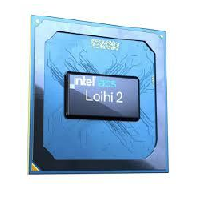
\includegraphics[width=0.65\columnwidth]{assets/images/Intel Lohi 2.png}
    \captionof{figure}{Intel Loihi 2}
\end{minipage}
  \end{center}
\vspace{-0.35em}

  \subsubsection*{The Cambridge Hafnium Oxide Memristor (2026)}
  The most commercially significant 2026 hardware development is the \textbf{University of Cambridge's hafnium
  oxide (\(\mathrm{HfO_2}\)) memristive synapse}. Unlike prior memristors relying on unstable conductive filament formation,
  this device exploits engineered \textbf{p-n heterointerfaces} between strontium-titanium-doped \(\mathrm{HfO_2}\) layers for
  deterministic, repeatable switching. Key measured properties:
  \begin{itemize}
    \item \textbf{70\% AI energy reduction} vs. conventional digital hardware.
    \item Switching currents \(\leq \mathbf{10^{-8}\,A}\)---one million times lower than standard oxide memristors.

    \item \textbf{Hundreds of stable conductance levels} for high-precision analogue in-memory computation

    \item Robust across \textbf{tens of thousands of switching cycles}.
  \end{itemize}
  The decisive commercial advantage: \(\mathrm{HfO_2}\) is already a standard gate dielectric in sub-10nm CMOS processes,
  meaning these synapses require \textbf{no new foundry infrastructure}---the single largest barrier to memristor
  commercialization, now eliminated.

  \begin{center}
\vspace{-0.5em}
\begin{minipage}{0.98\columnwidth}
\centering
    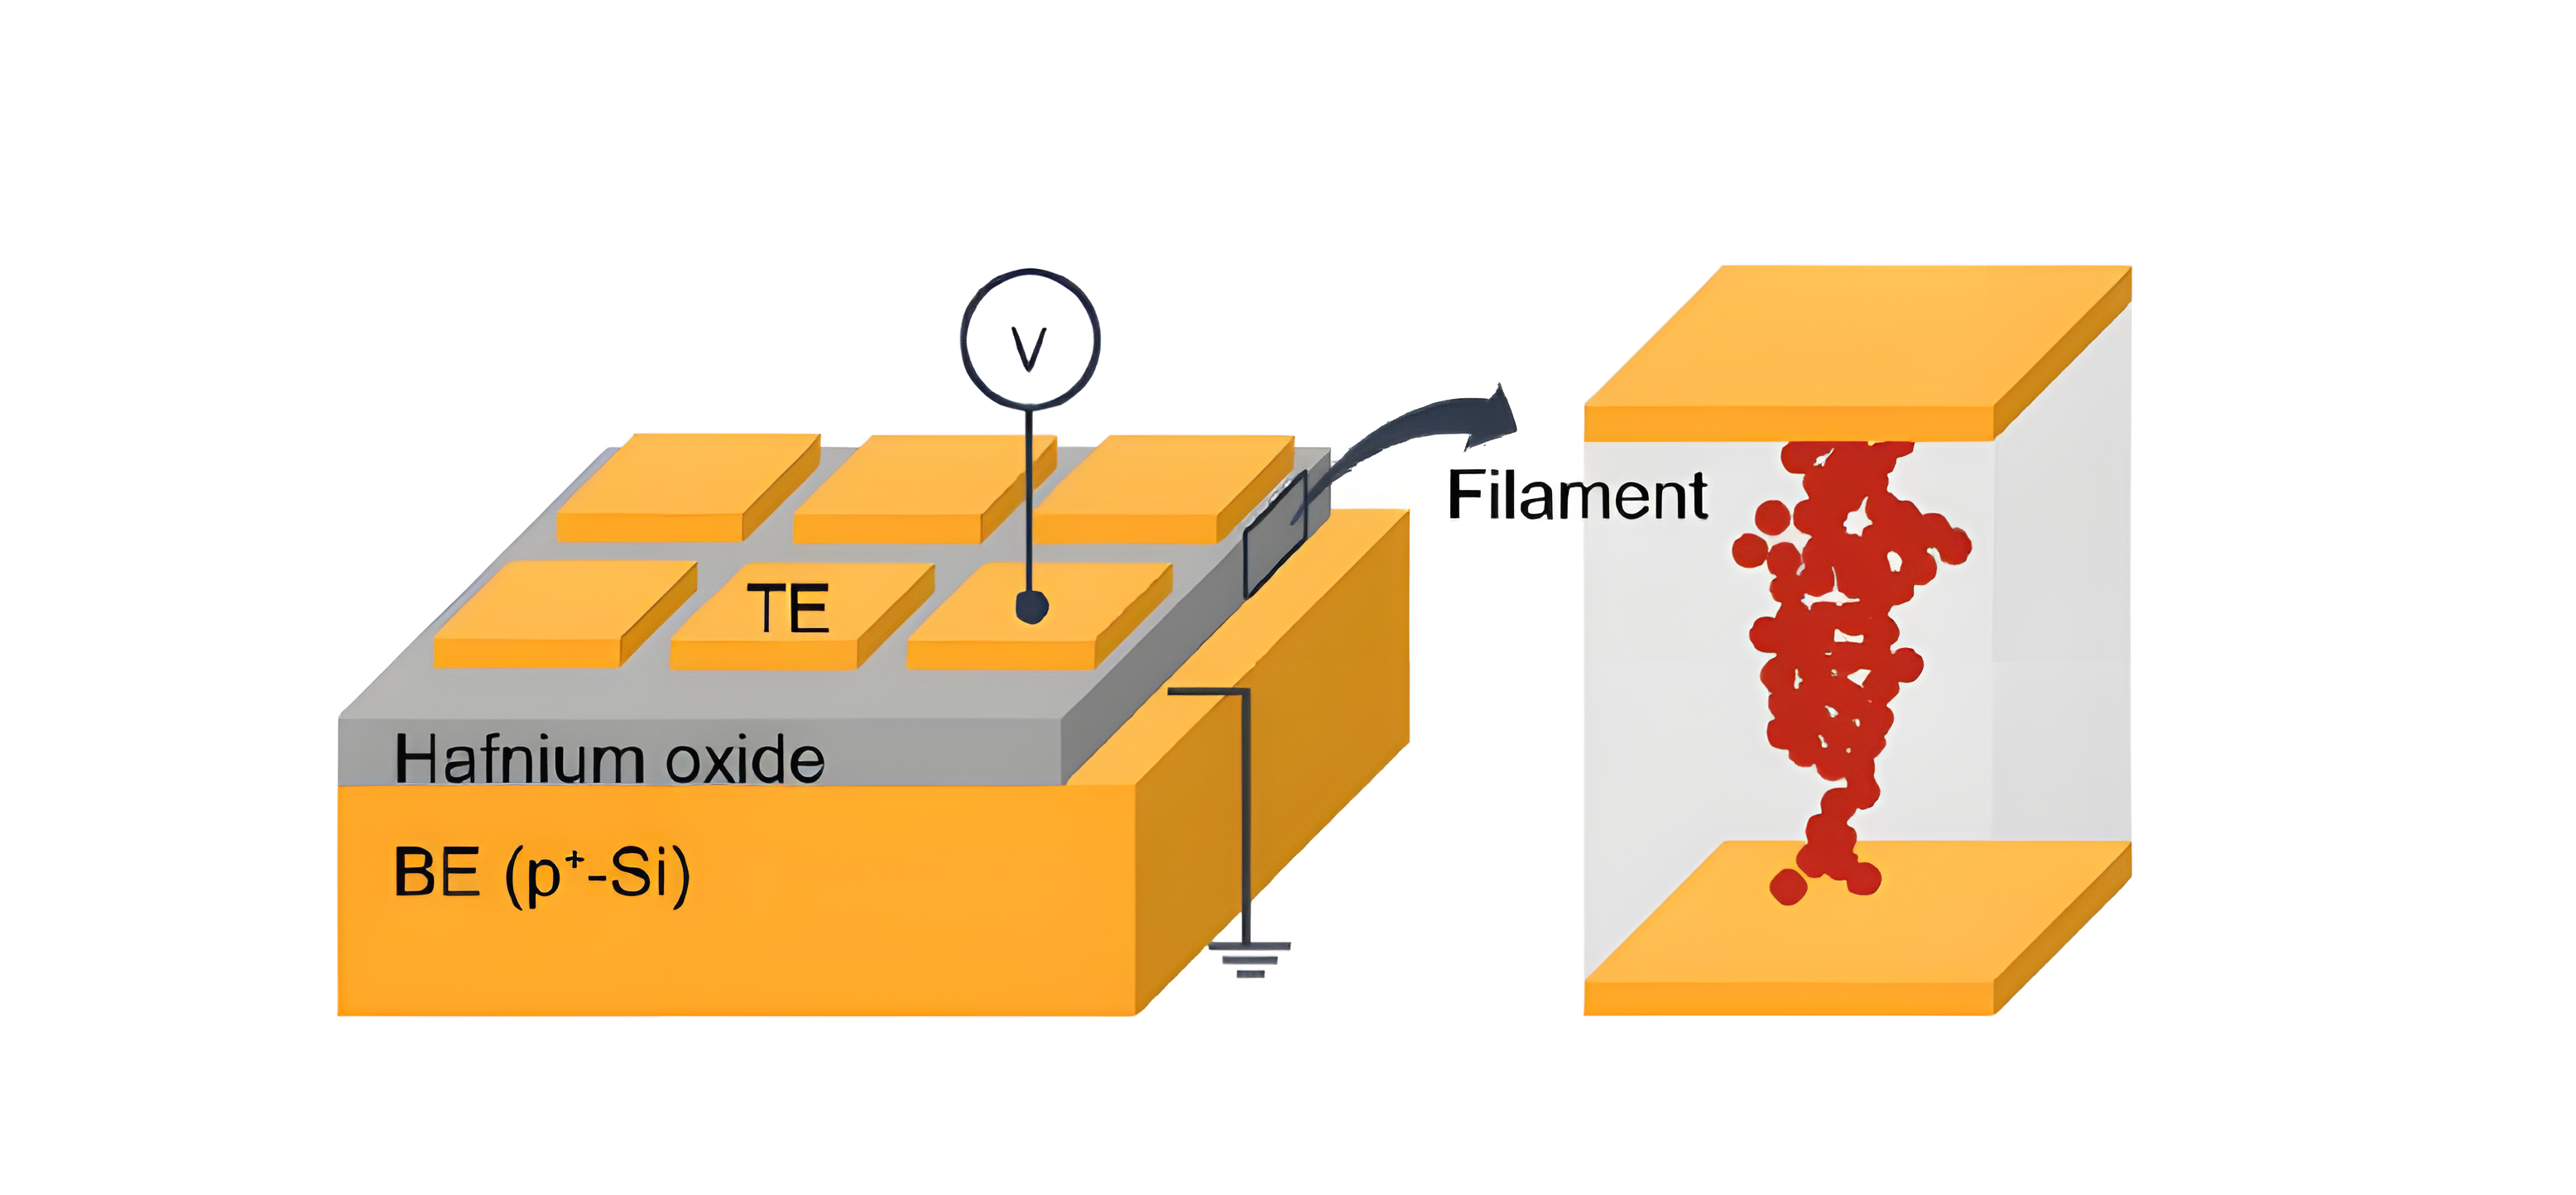
\includegraphics[width=0.85\columnwidth]{assets/images/Hafnium Oxide Memristor.png}
    \captionof{figure}{Hafnium Oxide Memristor}
\end{minipage}
  \end{center}
\vspace{-0.35em}

  \subsubsection*{The Integration Challenge: Bridging Spikes and Silicon Pipelines}
  Deploying neuromorphic accelerators within real engineering systems requires solving a fundamental interface
  problem: \textbf{neuromorphic hardware speaks in spikes; conventional software speaks in floating-point
  numbers}.

  \noindent
  The practical integration pipeline involves three stages:
  \begin{enumerate}
    \item \textbf{Encoding:} Real-valued sensor data (images, audio, signals) must be converted to spike trains---either
      via Poisson rate encoding, temporal coding, or, most efficiently, the differential coding scheme from
      ICML 2025
    \item \textbf{Processing:} The spiking accelerator (e.g., Loihi 2) processes the spike representation using on-chip
      LIF neurons and local learning rules
    \item \textbf{Decoding:} Output spike patterns must be decoded back to class labels, regression outputs, or control
      signals usable by downstream conventional systems
  \end{enumerate}

  \subsection*{\centering\uppercase{Market Trajectory and Commercialization Roadmap}}
  The commercial momentum behind neuromorphic computing is unambiguous and accelerating. The global
  market is projected to grow from \textbf{\$2.6 billion (2024) to \$61.48 billion by 2035} at a CAGR of \textbf{33.32\%}---
  among the fastest expansion trajectories in semiconductor history. Patent filings surged \textbf{401\% through early
  2026} with 596 filings recorded, driven by Intel, IBM, Samsung, and emerging neuromorphic startups.

  \noindent
  \begin{justify}
    The \textbf{2025 Neuromorphic Computing Roadmap} outlines three commercialization phases:
    \begin{itemize}
      \item \textbf{2025--2027:} Narrow-task edge deployment---always-on sensing, anomaly detection, IoT.
      \item \textbf{2027--2030:} Hybrid neuromorphic-GPU co-processors---SNN accelerators handling temporal data within conventional AI pipelines.
      \item \textbf{2030+:} Fully autonomous neuromorphic AI workloads with standardized programming models.
    \end{itemize}
  \end{justify}
  The roadmap explicitly identifies \textbf{benchmark standardization} as the field's highest-priority systemic challenge
  without MLPerf-equivalent metrics for SNNs, hardware vendors cannot make credible performance claims to
  enterprise buyers.
  \subsection*{\centering\uppercase{Conclusion}}
  Neuromorphic computing has crossed from architectural curiosity to measurable engineering reality. In 2024--2025,
  SNNs trained with surrogate gradients and MFT achieved ImageNet accuracies competitive with
  conventional deep learning. SpikeYOLO delivered object detection accuracy 15\% above prior SNN state-of-the-
  art with \(5.7\times\) energy savings. Advanced SpikingYOLOX brought transformer-class capability to spike-domain
  vision. On the hardware side, Hala Point's billion-neuron system operates at \(100\times\) lower power than GPU
  equivalents, while Cambridge's hafnium oxide memristors offer a 70\% energy cut using foundry-compatible
  materials.

  \noindent
  The remaining challenges memristor thermal stability, SNN algorithm scalability to transformer-scale models,
  and software toolchain fragmentation are real but tractable, with active research on each front in 2025 and 2026.
  For the electronics engineer of tomorrow, neuromorphic computing is no longer a specialization to consider. It is
  a foundation to master. The brain did not evolve over millions of years only to be ignored by its own imitations.

  \subsection*{\centering\uppercase{References}}
  \begin{justify}
  \Urlmuskip=0mu plus 1mu\relax
  \begin{enumerate}
    \item X. Luo et al., "Integer-Valued Training and Spike-Driven Inference Spiking Neural Network for High-
      Performance Object Detection," in Proc. ECCV, 2024. [Online]. Available:
      \url{https://eccv.ecva.net/virtual/2024/poster/150}

    \item ACM, "Advanced SpikingYOLOX: Extending Spiking Neural Network on Object Detection with
      Spike-based Partial Self-Attention and 2D-Spiking Transformer," in Proc. ACM MM, 2025. DOI:
      \url{10.1145/3746027.3754854}

    \item Y. Wang et al., "Deep Spiking Neural Networks Based on Model Fusion Technology," Engineering
      Applications of AI, Feb. 2025. DOI: \url{10.1016/j.engappai.2024.109873}

    \item ICML, "Differential Coding for Training-Free ANN-to-SNN Conversion," in Proc. ICML, 2025.
      [Online]. Available: \url{https://icml.cc/virtual/2025/poster/45408}

    \item OpenReview, "Error-Free ANN-to-SNN Conversion for Extreme Edge Efficiency," Jan. 2025.
      [Online]. Available: \url{https://openreview.net/forum?id=GTzP2GC7NR}

    \item Intel Corporation, "Intel Builds World's Largest Neuromorphic System---Hala Point," Intel
      Newsroom, Apr. 2024. [Online]. Available: \url{https://newsroom.intel.com}

    \item University of Cambridge, "\(\mathrm{HfO_2}\)-based Memristive Synapses via Asymmetric p-n
      Heterointerfaces," Science Advances, Mar. 2026.
  \end{enumerate}
  \end{justify}
\end{multicols}